\documentclass[../main.tex]{subfiles}

%\graphicspath{{\subfix{../images/}}}

\begin{document}

\section{{\sc Mattuck} - A giude to Feynman diagrams in the Many-Body problem}

\section{{\sc Fetter, Walecka} - Quantum Theory of Many-Particle Systems}
\subsection{2.2 Equation of state for an ultrarelativistic ideal gas}
\begin{align}
\epsilon_p
&=\lim_{p\gg m_0c}\sqrt{(pc)^2+m_0^2c^4}\\
&=pc\sqrt{1+\frac{m_0^2c^2\cdot c^2}{p^2\cdot c^2}}\\
&\approx pc
\end{align}
Quick thermodynamics review
\begin{align}
\text{1st law}\quad dU&=\delta Q+\delta W\\
\text{2nd law}\quad dS&=dS_i+\frac{\delta Q}{T}, \qquad dS_i>0\\
\text{Gibbs Fund.Form}&\rightarrow dS=\frac{1}{T}dU-\frac{1}{T}\delta W=\frac{1}{T}dU+\frac{1}{T}\sum_i y_idX_i\\
&\rightarrow \left.\frac{dS}{dU}\right|_{X_i}=\frac{1}{T}\qquad\rightarrow\qquad U=U(T,X_i)\\
&\rightarrow \left.\frac{dS}{dX_i}\right|_{U,X_j}=\frac{y_i}{T}\qquad\rightarrow\qquad y_i=y_i(T,X_j)
\end{align}

\section{{\sc Coleman} - Introduction to Many-Body Physics}
\subsection{Problem 2.1 - Specific heat capacity of a solid}
Using the Boltzmann statistics and $E_n=\hbar\omega(n+\frac{1}{2})$ the energy $E$ of a system of $N_\text{AV}$ harmonic oscillators (in 3d!!) is given by 
\begin{align}
    E
    &=3N_{AV}\frac{\sum_nE_ne^{-\frac{E_n}{k_BT}}}{\sum_ne^{-\frac{E_n}{k_{B}T}}}\\
    &=3N_{AV}\frac{\sum_n\left(\hbar\omega\left[n+\frac{1}{2}\right]\right)e^{-\frac{n\hbar\omega}{k_BT}}e^{-\frac{\hbar\omega}{2k_BT}}}{\sum_ne^{-\frac{n\hbar\omega}{k_BT}}e^{-\frac{\hbar\omega}{2k_BT}}}\\
    &=3N_{AV}\hbar\omega\left(\frac{1}{2}+\frac{\sum_n ne^{-\frac{n\hbar\omega}{k_BT}}}{\sum_ne^{-\frac{n\hbar\omega}{k_BT}}}\right)\\
    &=3N_{AV}\hbar\omega\left(\frac{1}{2}+\frac{1}{e^{\frac{\hbar\omega}{k_BT}}-1}\right)
\end{align}
where we used the sum formulas
\begin{align}
    s_1&=\sum_{n=0}q^n=\frac{1}{1-q}\\
    s_2&=\sum_{n=0}nq^n=q\frac{ds_1}{dq}=\frac{q}{(1-q)^2}
\end{align}
the specific heat can the be calculated as
\begin{align}
    C_V&=\frac{dE}{dT}\\
    &=3N_{AV}\hbar\omega\frac{\exp\left[\frac{\hbar\omega}{kT}\right]\frac{\hbar\omega}{kT^2}}{\left[\exp\left[\frac{\hbar\omega}{kT}\right]-1\right]^2}\\
    &=3N_{AV}k\frac{x^2\exp(x)}{\left[\exp(x)-1\right]^2}\\
    &=3N_{AV}k\frac{x^2}{\left[\exp(x/2)-\exp(-x/2)\right]^2}\\
    &=3N_{AV}k\frac{x^2}{\left[\exp(x/2)-\exp(-x/2)\right]^2}\\
    &=3N_{AV}k\left(\frac{x/2}{\sinh(x/2)}\right)^2\\
\end{align}
The Dulong-Petit rule says $k/2$ per harmonic degree of freedom which means in 3d that $C_V/N=3k$ (for each harmonic degree there is also a kinetic one - so $f=6$ )
\begin{center}
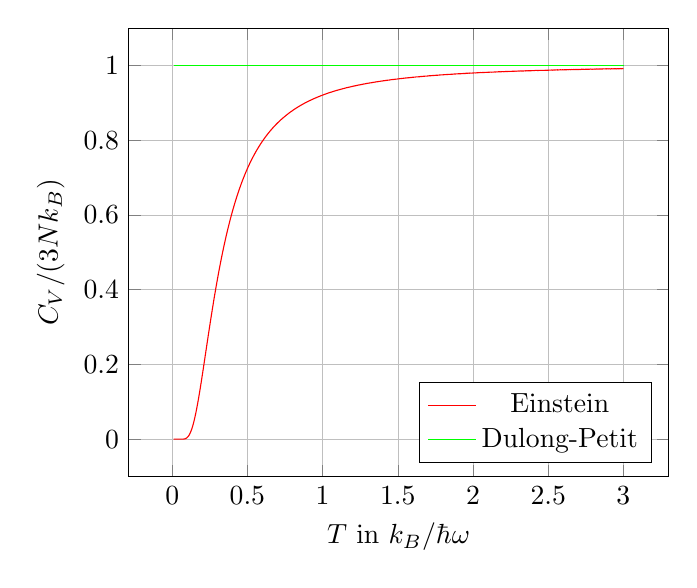
\begin{tikzpicture}
\begin{axis}[
    xlabel = $T$ in $k_B/\hbar\omega$,
    ylabel = {$C_V/(3Nk_B)$},
    legend pos=south east,
    grid=both,
    grid style={line width=.1pt, draw=gray!10},
    major grid style={line width=.2pt,draw=gray!50}]
\addplot[color=red,domain=0.01:3, samples=1000, ]{((1/(2*x))/(sinh(1/(2*x))))^2};
\addlegendentry{Einstein}
\addplot[color=green,domain=0.01:3, samples=1000, ]{1};
\addlegendentry{Dulong-Petit}
\end{axis}
\end{tikzpicture}
\end{center}

\end{document}